
\newpage


\chapter{Robot de pruebas}
\label{chap:robot}

Con la finalidad de demostrar y hacer un primer uso de la aplicación RobotUI se ha decidido abordar la elaboración de un vehículo de pruebas. Dicho vehículo será utilizado de modelo o guía para el 
resto de personas que quieran crear un robot para su integración en la aplicación o bien para programar un robot del que ya dispongan previamente.\\

En el presente capítulo se detalla los diferentes pasos que se han seguido a la hora de la construcción y programación del vehículo desarrollado. Este capítulo tiene como objetivo proporcionar al usuario
una guía básica a partir de la cual poder desarrollar sus propios robots e integrarlos en la aplicación RobotUI.\\


\begin{figure}[H]
  \begin{center}
    \includegraphics[scale=0.2]{imagenes/robot2.jpg}
  \end{center}
  \caption{Imagen del robot de pruebas desarrollado.}
  \label{robot:robot02}
\end{figure}


\section{Análisis}
\label{sec:analisis}

\subsection{Análisis de requerimientos hardware}
\label{sec:requerimientos-hardware}

Se ha optado por la construcción de un  pequeño robot móvil dotado de un chasis de 4 ruedas donde cada una de ellas está accionada por un motor. Los motores seleccionados deberán funcionar a 
corriente continua de manera que en función de la polarización de los terminales haga girar las ruedas en una dirección o la contraria (marcha adelante o atrás).\\

El chasis utilizado deberá permitir añadir multitud de componentes necesarios para construir el robot, deberá disponer de paneles para instalar las diferentes
placas electrónicas y sensores.\\

El robot además necesita de una cámara para la obtención de vídeo y su transmisión siendo necesaria una cámara de pequeñas dimensiones de alta definición.\\

Por otra parte, todo robot necesita de una unidad de central de procesamiento donde se localizará el programa de control. Este programa tendrá la función de interpretar las diferentes señales recibidas,
control de sensores y dispositivos conectados. Además, esta placa es la encargada de distribuir la alimentación por los diferentes componentes hardware que lo necesiten y recibir las señales de
los sensores y enviarla a los motores. Utilizando para ello la placa Raspberry Pi modelo B cuya descripción se encuentra en la sección \ref{sec:raspberry}.\\

Este modelo de placa dispone de  una serie de pines denominados GPIO (General Purpose Input/Output) que son, como su propio nombre indica, un sistema de E/S (Entrada/Salida) de propósito general,
es decir, una serie de conexiones que se pueden usar como entradas o salidas para usos múltiples. Estos pines están incluidos en todos los modelos de Raspberry Pi, con la
finalidad de ser utilizados en diferentes proyectos de una manera similar a la que se haría con Arduino\footnote{Arduino es una plataforma de prototipos electrónica de código abierto (open-source) 
basada en hardware y software flexibles y fáciles de usar.}.

\section{Análisis de requerimientos de Software}

Habiendo detallado los requerimientos hardware para la construcción del robot, pasamos al análisis de los diferentes requerimiento software para la correcta
gestión de los diferentes elementos hardware y para su correcto funcionamiento.\\

En cuanto a la programación del robot, uno de los requisitos fundamentales es el de disponer de una vía de comunicación bidireccional.\\

Para ello se ha seleccionado el entorno de ejecución Node.Js, el cual permite escribir programas en JavaScript además de disponer de una gran cantidad de bibliotecas hechas por toda una comunidad que la respalda.
Además de que permite escribir programas relativamente complejos en tan sólo unas pocas líneas de código.\\

se ha realizado haciendo uso de Websockets los cuales presentan algunas ventajas sobre simples solicitudes http:

\begin{itemize}
 \item Velocidad: Una petición http normal tiene que establecer una conexión antes de comenzar las transacciones, la cual toma bastante tiempo. 
 Los Websockets, una vez establecida la conexión, siempre están abiertos y listos para enviar o recibir datos. Esto significa que el retraso puede ser tan bajo como su ping,
 en torno a un milisegundo o dos en la mayoría de los casos.
 \item Bidireccional: Los Websockets permiten transmisión de datos en ambas direcciones permitiendo la activación de eventos en el cliente y viceversa.
\end{itemize}

Como podemos ver las propiedades anteriormente descritas resultan esenciales para nuestro proyecto que, como cabe recordar, queremos realizar lectura de sensores y envío de órdenes desde un servidor 
externo. Además de la transmisión de vídeo.\\

\section{Montaje}

En esta sección se recogen todas las descripciones y procedimientos seguidos y que han resultado de mayor interés a la hora de la construcción del robot y sus diferentes interconexiones.\\

\subsection{Interconexión de elementos}

En el presente punto, se recoge todos aquellos puntos de interés referentes a la interconexión de elementos utilizados, los cuales quedaron descritos en la sección \emph{Tecnologías hardware}
\ref{sec:tecnologias-hardware} junto con sus especificaciones.\\

Comenzando por el módulo central del sistema, la placa Raspberry Pi Model B+, dispone de una serie de pines denominados GPIO (General Purpose Input/Output) es, como su propio nombre indica, 
un sistema de E/S (Entrada/Salida) de propósito general, es decir, una serie de conexiones que se pueden usar como entradas o salidas para usos múltiples. Estos pines se encuentran en todos
los modelos de Raspberry Pi.\\

Los GPIO representan la interfaz entre la Raspberry Pi y el mundo exterior. En este caso para el control de los motores del vehículo.\\

Primeramente, antes de comenzar a utilizarlos debemos conocer sus características y como están distribuidos en nuestra placa. los pines GPIO para la Raspberry Pi 3 Model B, se encuentran distribuidos 
de la siguiente manera:

\begin{figure}[H]
  \begin{center}
    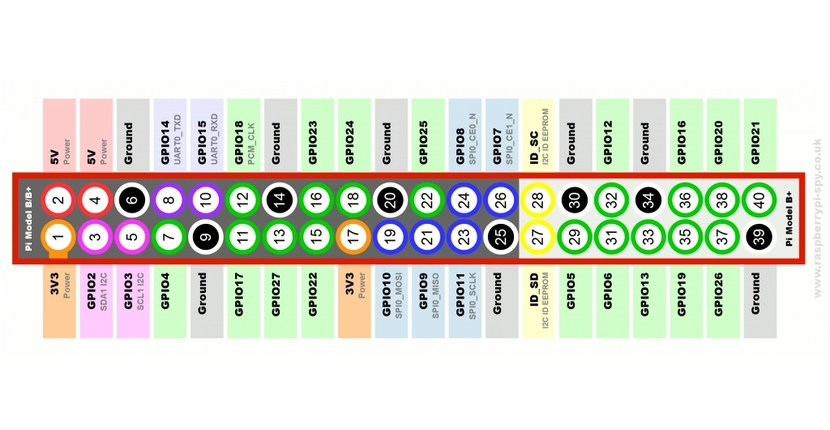
\includegraphics[scale=0.4]{imagenes/robot/gpio-conexiones.jpg}
  \end{center}
  \caption{Esquema GPIO de una Raspberry Pi Model B+.}
  \label{gantt:tareas01}
\end{figure}

Los pines empleados son los siguientes para la construcción del robot han sido los siguientes:\\

\begin{table}[H]
  \begin{center}
    \begin{tabular}{|p{2.5cm}|p{2.5cm}|p{4.5cm}|}
      \hline
      {\textbf{GPIO}} & \textbf{ Modo } & \textbf{ Control }\\
      \hline
      {\textbf{ 2 }} & { OUTPUT } & { Motores lado izquierdo }  \\
     \hline
      {\textbf{ 3 }} & { OUTPUT } & { Motores lado izquierdo } \\
      \hline
      {\textbf{ 17 }} & { OUTPUT } & {  Motores lado derecho } \\
      \hline
      {\textbf{ 27 }} & { OUTPUT } & { Motores lado derecho } \\
     \hline   
    \end{tabular}
  \end{center}
\caption{ Tabla con los puertos GPIO utilizados, su configuración establecida y su utilización. }
\end{table}


Pero existe una problemática y es que no podemos conectar directamente los pines de salida de nuestra placa Raspberry Pi directamente a los motores. Esto es debido a
que la placa no dispone de potencia suficiente para mover actuadores. De hecho, la función de la placa no debe ser ejecutar acciones sino mandar ejecutar acciones a drivers que realicen
el trabajo pesado.\\

Para ello empleamos el L298N, un controlador (driver) de motores, el cual nos permite encender y controlar dos motores de corriente continua desde una Raspberry Pi, Arduino o cualquier placa similiar,
variando tanto la dirección como la velocidad de giro.\\

La corriente máxima que el L298N puede suministrar a los motores es, en teoría, 2A por salida (hasta 3A de pico) y una tensión de alimentación de 3V a 35V. Sin embargo, el L298N tiene una 
eficiencia baja. La electrónica supone una caída de tensión de unos 3V, es decir, la tensión que recibe el motor es unos 3V inferior a la tensión de alimentación.\\

Estas pérdidas se disipan en forma de calor lo que se traduce en que, a efectos prácticos, es difícil que podamos obtener más de 0.8-1A por fase sin exceder el rango de temperatura de funcionamiento.\\

El L298N incorpora protecciones contra efectos que pueden producirse al manejar motores de corriente continua. Dispone de protecciones contra sobre intensidad, sobre temperatura, y diodos de protección
contra corrientes inducidas.\\

El módulo seleccionado, el cual incorpora el controlador L298N, cuenta con todos los componentes necesarios para funcionar sin necesidad de elementos adicionales, entre ellos diodos de protección
y un regulador \textbf{LM7805} que suministra 5V a la parte lógica del integrado L298N. Además cuenta con jumpers de selección para habilitar cada una de las salidas del módulo (A y B).
La \textbf{salida A} esta conformada por \textbf{OUT1} y \textbf{OUT2} y la \textbf{salida B} por \textbf{OUT3} y \textbf{OUT4}. Los pines de habilitación son \textbf{ENA} y \textbf{ENB} respectivamente.\\

En la figura \ref{diagrama:L298N-salidas} se muestra el módulo empleado con sus diferentes pines al detalle.\\


\begin{figure}[H]
  \begin{center}
    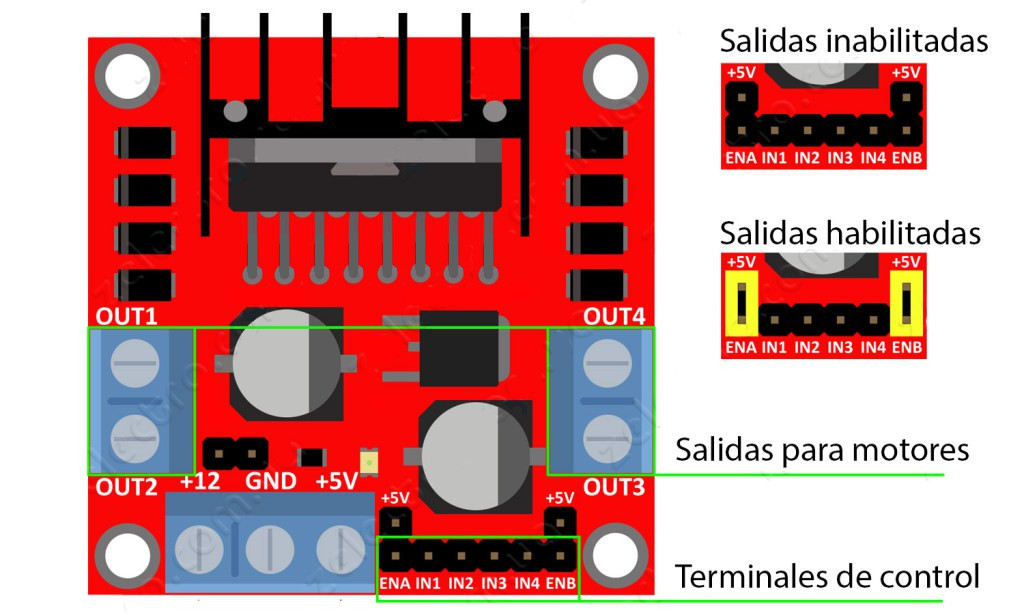
\includegraphics[scale=2.5]{imagenes/L298N-conexiones.jpg}
  \end{center}
  \caption{Pines de entrada/salida del módulo L298N empleado.}
  \label{diagrama:L298N-salidas}
\end{figure}

\subsubsection{Alimentación}

Para la alimentación del conjunto se ha optado por la utilización de dos baterías. Una para dotar de energía a la placa de control y otra para la alimentación de los motores debido a la gran cantidad de energía 
que éstos demandan y su elevado consumo.\\

Para la alimentación de la placa Raspberry Pi, se ha optado por la utilización de una batería de Litio desarrollada específicamente para su uso con este modelo de placas el cual permite una integración
perfecta. Dicho módulo de alimentación queda descrito en la subapartado correspondiente de herramientas utilizadas \ref{componente:bateria-expansion}.

Imagen de la Raspberry Pi junto con su módulo de expansión de batería:

\begin{figure}[H]
  \begin{center}
    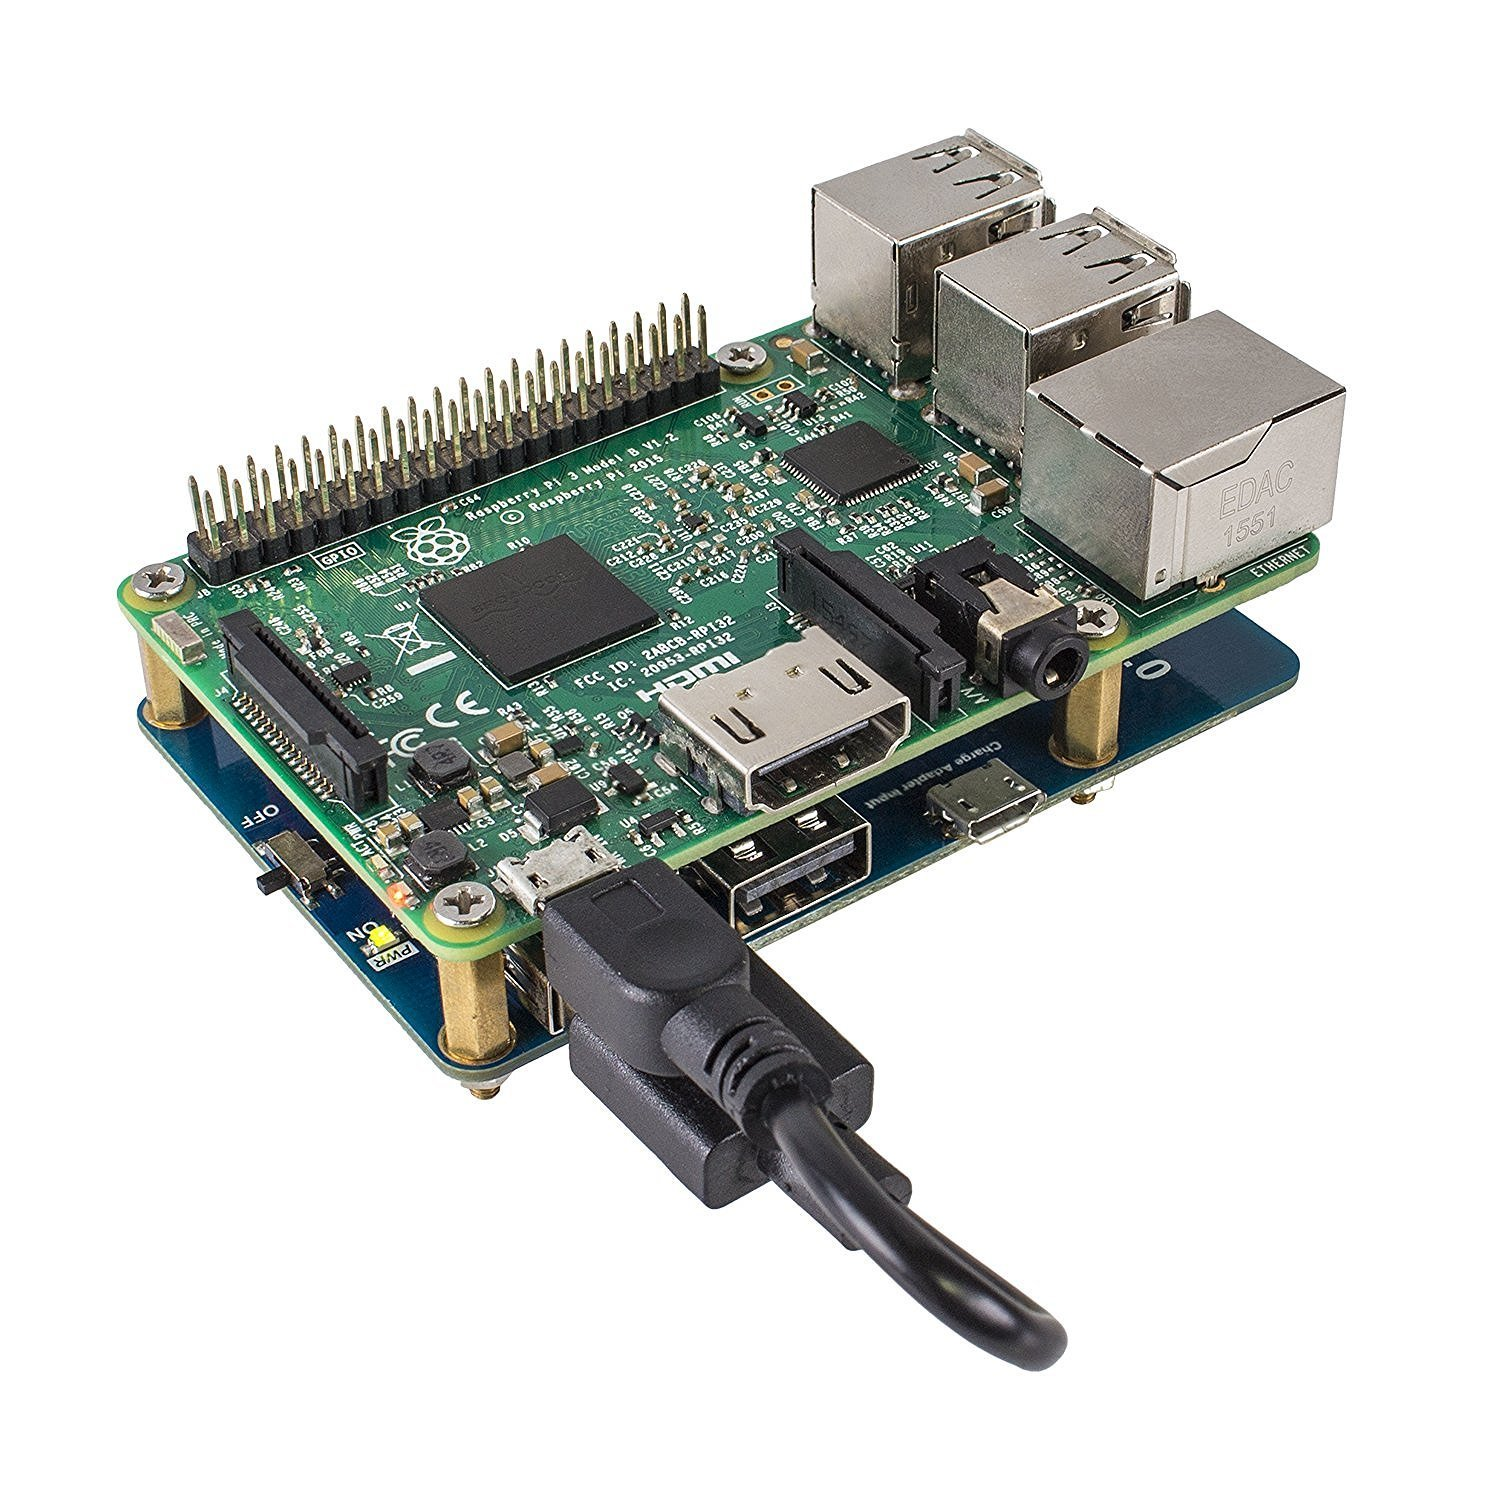
\includegraphics[scale=0.15]{imagenes/modulo-expansion-rpi.jpg}
  \end{center}
  \caption{Conjunto Raspberry Pi y módulo de expansión de alimentación.}
  \label{figura:rpi-modulo-bateria}
\end{figure}


Imagen de la batería LiPo para la alimentación de los motores:


\begin{figure}[H]
  \begin{center}
    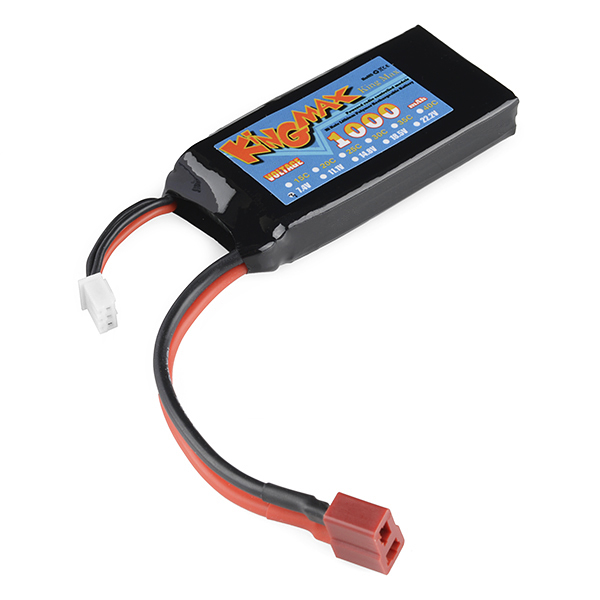
\includegraphics[scale=0.4]{imagenes/robot/bateria-lipo.jpg}
  \end{center}
  \caption{Vista de la batería LiPo que alimenta los motores.}
  \label{figura:rpi-modulo-bateria}
\end{figure}



\subsubsection{Esquema de conexiones}

El siguiente gráfico \ref{diagrama:esquema-conexiones} muestra las conexiones de todo el conjunto:

\begin{figure}[H]
  \hspace*{.5in}{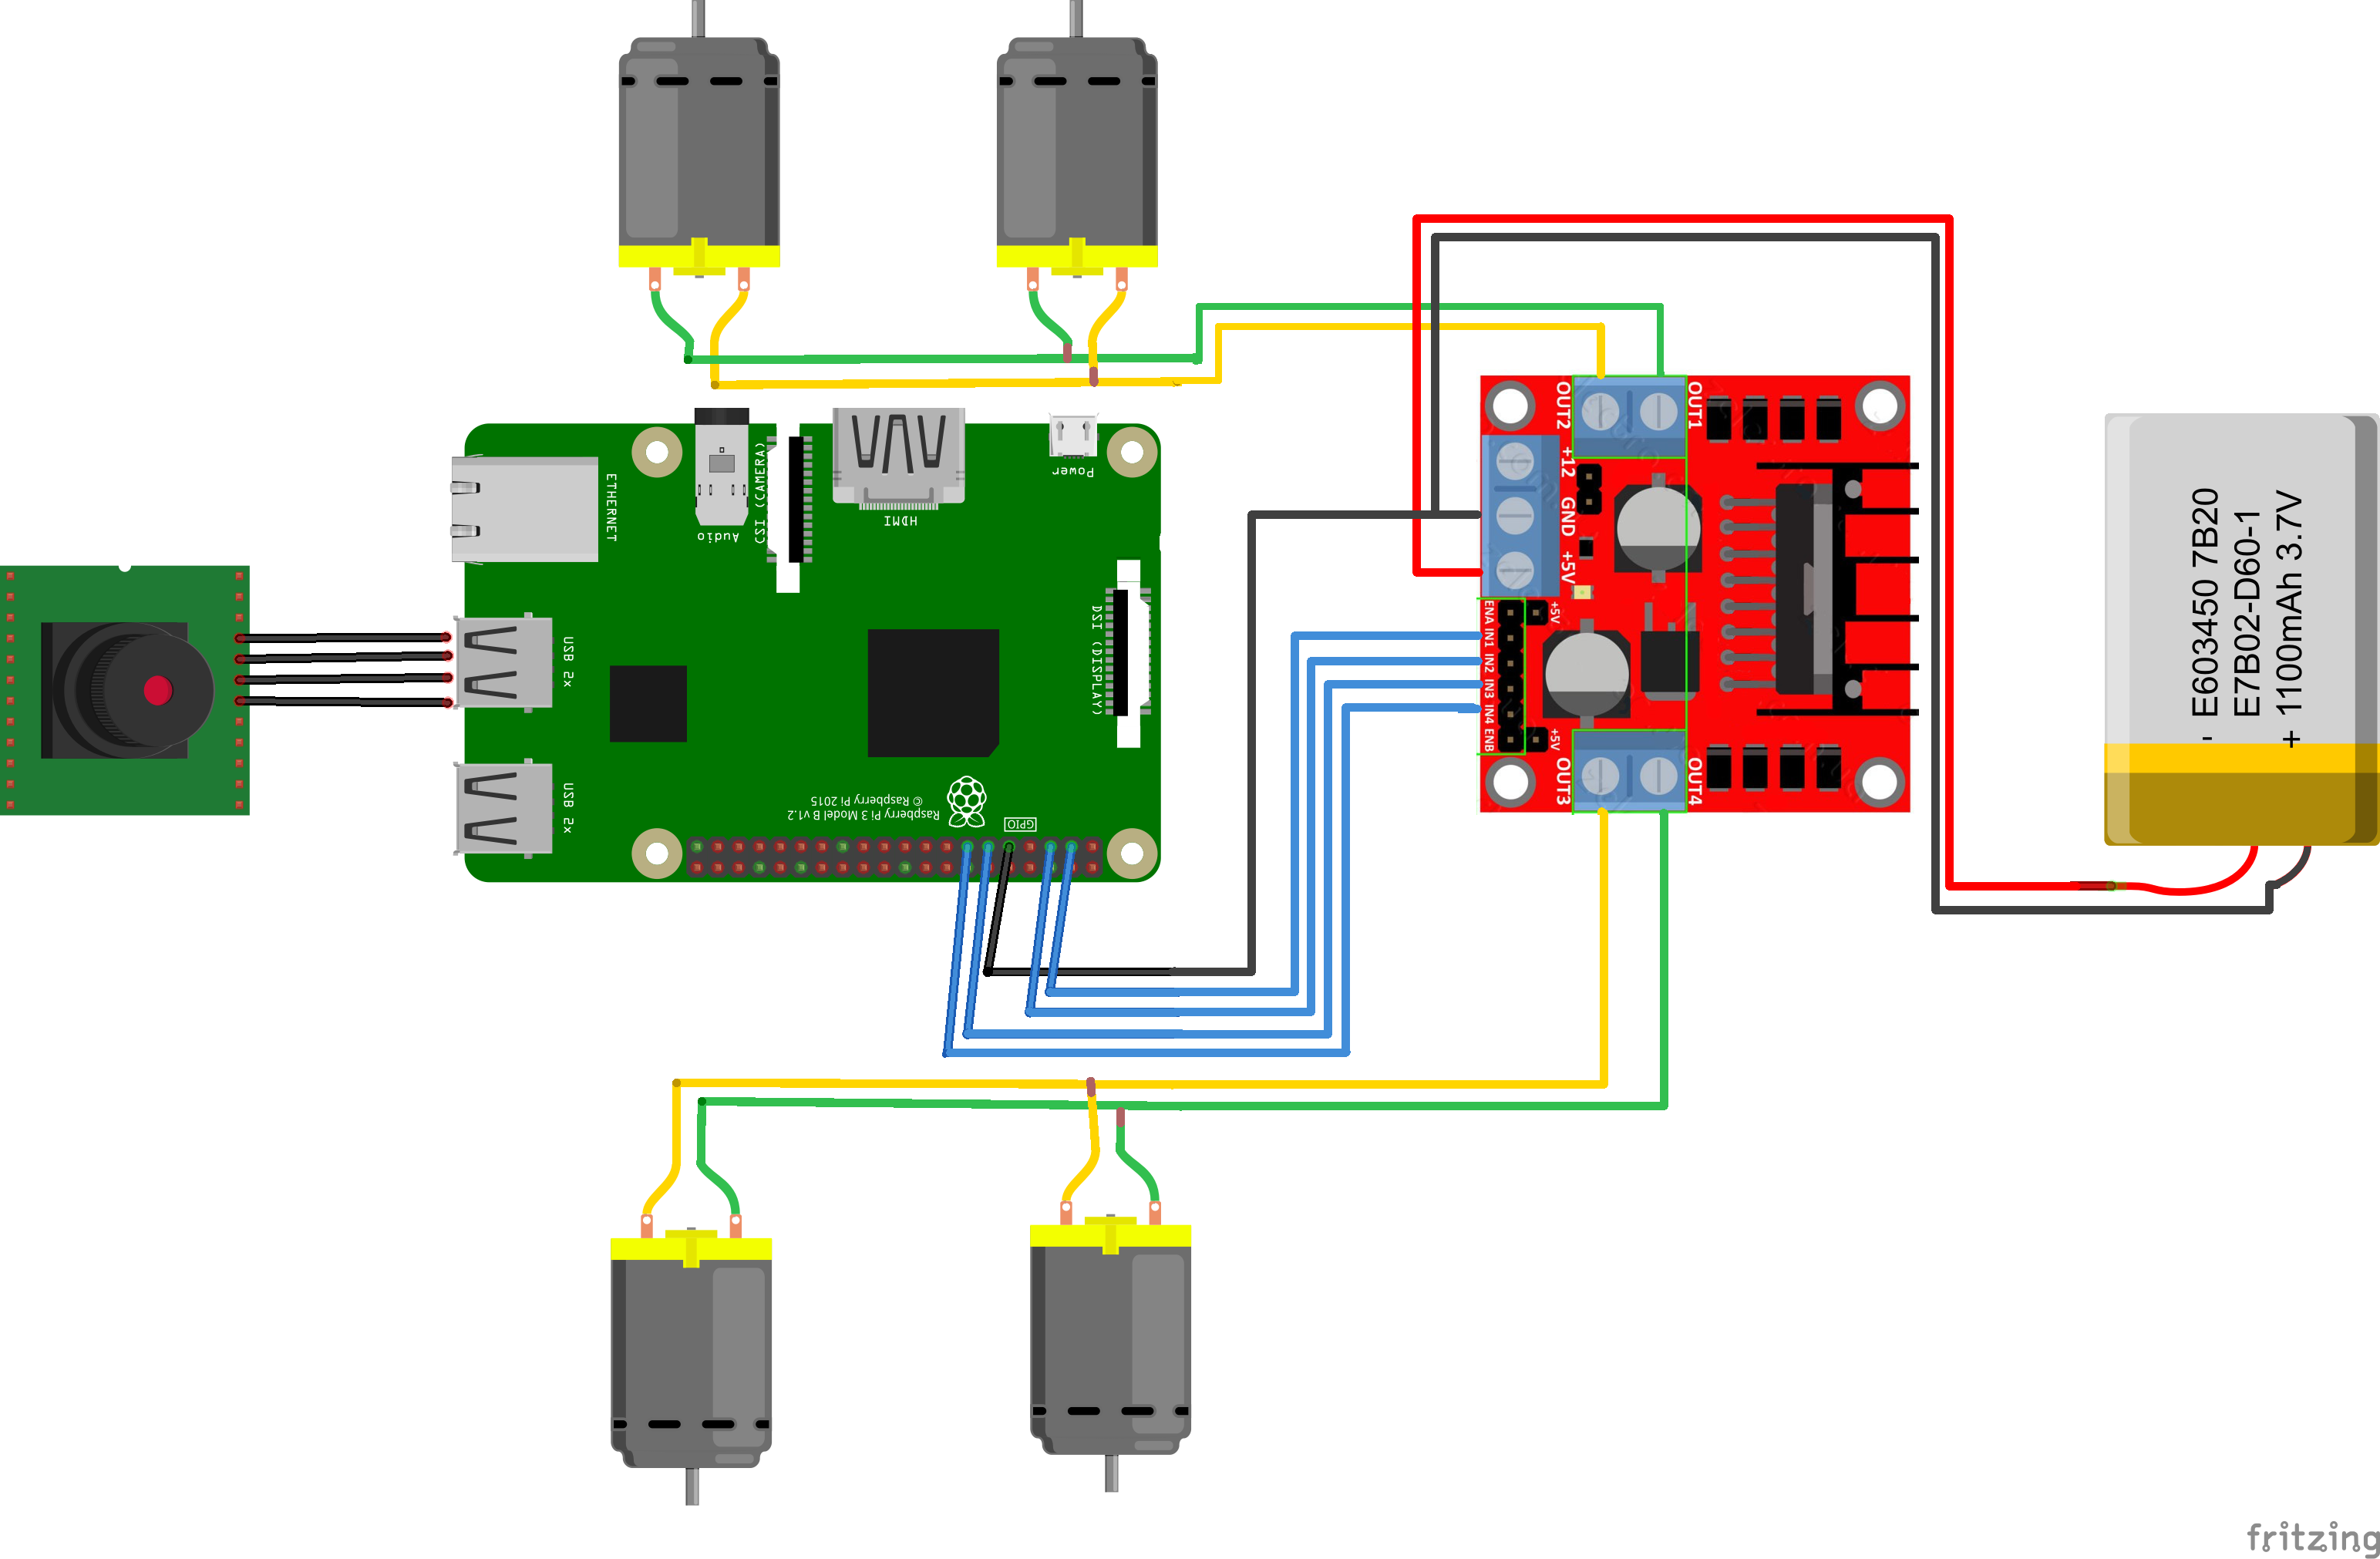
\includegraphics[scale=0.65,angle=270]{imagenes/robot/robot-esquema2.png}}
  \caption{Esquema de conexiones del robot de pruebas.}
  \label{diagrama:esquema-conexiones}
\end{figure}


\begin{figure}[H]
  \begin{center}
    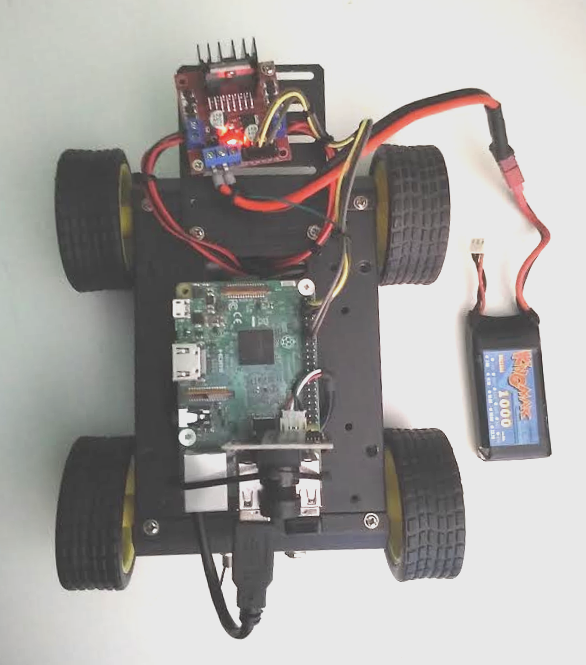
\includegraphics[scale=0.4]{imagenes/robot/robot-bateria-lipo.png}
  \end{center}
  \caption{Vista superior del vehículo.}
  \label{figura:rpi-modulo-bateria}
\end{figure}

    
\section{Software de control}
  

Para la programación del robot se ha empleado el lenguaje de programación JavaScript en un entorno de ejecución Node.js. A continuación se describirá aquellos aspectos más importantes
referentes al código desarrollado para el control del robot.\\

Primeramente se ha realizado la carga de librerías necesarias, entre ellas encontramos:

\begin{itemize}
 \item \emph{pigpio}: Módulo para la comunicación y control de los pines GPIO.
 \item \emph{child process}: El módulo child\_process proporciona la capacidad de generar procesos secundarios. Se ha empleado para la captura de vídeo mediante el lanzado de comandos ffmpeg.
 \item \emph{socket.io}: Biblioteca que establece enlaces bidireccionales en tiempo real y en comunicación basada por eventos.
\end{itemize}


\subsection{Entrada/Salida}

En segundo lugar se han definido los diferentes pines GPIO a utilizar y si serán empleados como pines de entrada o de salida:

\begin{table}[H]
  \begin{center}
    \begin{tabular}{|p{2.5cm}|p{2.5cm}|p{4.5cm}|}
      \hline
      {\textbf{GPIO}} & \textbf{ Modo } & \textbf{ Control }\\
      \hline
      {\textbf{ 2 }} & { OUTPUT } & { Motores lado izquierdo }  \\
     \hline
      {\textbf{ 3 }} & { OUTPUT } & { Motores lado izquierdo } \\
      \hline
      {\textbf{ 17 }} & { OUTPUT } & {  Motores lado derecho } \\
      \hline
      {\textbf{ 27 }} & { OUTPUT } & { Motores lado derecho } \\
     \hline   
    \end{tabular}
  \end{center}
\caption{ Configuración establecida para los puertos GPIO. }
\end{table}


Si para el vehículo que deseemos programar resultan necesarios más pines para la utilización de servos, sensores o cualquier otro elemento, tan solo debemos inicializarlos e indicar si van a ser pines de entrada
o de salida. Si existen dudas al respecto se puede acceder a la documentación de la biblioteca \emph{pigpio} en el siguiente enlace: \url{https://www.npmjs.com/package/pigpio}.
Para el caso de este proyecto, la inicialización de los pines se ha realizado mediante las siguientes instrucciones:

\begin{lstlisting}[language=JavaScript]
  // Carga del módulo.
  var Gpio = require('pigpio').Gpio;

  // Pines utilizados. Motores izquierdos: 2 y 3, motores derechos: 17 y 27
  var gpio2 = new Gpio(2, {mode: Gpio.OUTPUT}),
    gpio3 = new Gpio(3, {mode: Gpio.OUTPUT}),
    gpio17 = new Gpio(17, {mode: Gpio.OUTPUT}),
    gpio27 = new Gpio(27, {mode: Gpio.OUTPUT});
\end{lstlisting}



\subsection{Comunicaciones}

En el punto anterior hemos visto las diferentes configuraciones de Entrada/Salida establecidas para el control de los diferentes motores y sensores. En el presente y sucesivos puntos describiremos los diferentes
canales de comunicación abiertos y los flujos de información existentes. En la figura \ref{figura:comunicaciones-robot} se muestra un gráfico representativo de los diferentes flujos de datos existentes:


\begin{figure}[H]
  \begin{center}
    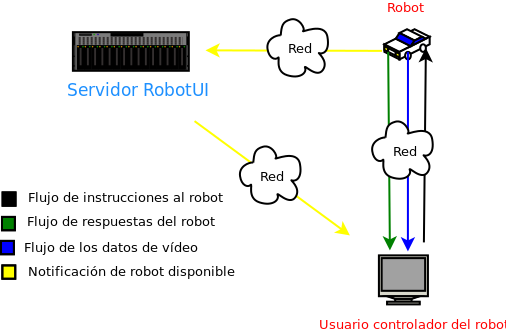
\includegraphics[scale=0.6]{diagramas/flujo-comunicaciones-robot.png}
  \end{center}
  \caption{Canales de comunicación abiertos por el robot.}
  \label{figura:comunicaciones-robot}
\end{figure}


Primeramente al accionar el robot, éste envía una notificación al servidor indicando que se encuentra en modo \emph{online} y permanece a la espera de que algún usuario de la aplicación decida conectarse para su control.
Canal de comunicación representado en amarillo en la figura \ref{figura:comunicaciones-robot}.\\

Un usuario ve disponible el robot y decide conectarse. Entonces se establece un enlace entre el robot, servidor, y el usuario, cliente. Flujo de comunicación representado en negro, figura \ref{figura:comunicaciones-robot}.\\

El usuario envía comandos al robot a través del canal abierto y las respuestas son enviadas a al cliente, transmisiones representados en verde para datos y en azul para el vídeo, figura \ref{figura:comunicaciones-robot}.\\

Las tres vías de comunicación entre el robot y el usuario discurren dentro de un mismo canal de comunicación (socket). En el siguiente punto se describirá más detalladamente el procedimiento.


\subsubsection{Sockets}

Ahora bien, una vez definidos los pines que activarán nuestros motores y los canales de comunicación necesitamos que éstos sean activados cuando desde una red externa lo indiquemos haremos uso
de la biblioteca Socket.io. Comenzamos el código incluyendo las librerías necesarias:

\begin{lstlisting}[language=JavaScript]
  var io_client = require('./node_modules/socket.io-client');
  var sails_client = require('./node_modules/sails.io.js');
\end{lstlisting}

Para la comunicaciones usuario y dispositivo robótico se ha empleado la biblioteca socket.io-client.\\

Para las comunicaciones directas con el servidor se ha empleado el SDK\footnote{Un kit de desarrollo de software o SDK (siglas en inglés de software development kit) es generalmente un conjunto de herramientas
de desarrollo de software que le permite al programador o desarrollador de software crear aplicaciones para un sistema concreto, por ejemplo ciertos paquetes de software, frameworks, etc.} proporcionado por el framework
para comunicarse con Sails a través de sockets desde una aplicación Node.js o desde el propio navegador.\\


El siguiente paso una vez cargadas las librerías es establecer las diferentes conexiones. El primer comportamiento deseado es, por parte del robot, lanzar un mensaje al servidor indicando su disponibilidad al servidor con la finalidad de
enviar las diferentes notificaciones a los usuarios que estén usando la aplicación. Para ello establecemos la conexión y enviamos un mensaje al servidor con el identificador del robot junto con su estado online igual a true. A continuación mostramos
el código:\\

\begin{lstlisting}[language=JavaScript]
  var io_server = sails_client(io_client);
  io_server.sails.url = 'http://46.101.102.33:80';
  io_server.socket.get('/robot/changetoonline/', {robot: '59188631c8e94ba54f7a4bdc', online: true});
\end{lstlisting}



Una vez realizado el paso anterior, tenemos un robot que ha indicado a la aplicación web principal de que se encuentra en estado online pero nada más. El siguiente paso sería establecer alguna comunicación que se mantuviera a la escucha a 
la espera de la llegada de nuevas conexiones. Para la creación del socket basta con la siguiente instrucción, la cual recibe un puerto que utilizará para mantenerse a la escucha:\\

\begin{lstlisting}[language=JavaScript]
  var io = require('./node_modules/socket.io').listen(8085, { log: false });
\end{lstlisting}


Con la finalidad de ir capturando los diferentes eventos, se han definido las siguientes funciones para la conexión y desconexión de los clientes:\\

\begin{lstlisting}[language=JavaScript]

io.sockets.on('connection', function (socket)
{

  //Almacenamiento del número total de clientes conectados.
  sockets[socket.id] = socket;
  console.log("Total clientes conectados : ", Object.keys(sockets).length);
  
  //Envío de un saludo.
  socket.emit('robotmsg', {msg: "!!!HOLA!!!"});


  //Salida de un cliente.
  socket.on('disconnect', function() {
    console.log('Bye!');
    stopStreaming(socket);
  });  
  
}
\end{lstlisting}

Cuando un evento \emph{action} es recibido se activada la función que procesa el comando recibido y activa las salidas correspondientes, la cual establece los pines necesarios a los valores
1 o 0 según el parámetro establecido. La tabla \ref{table:table-pin-out} muestra las diferentes combinaciones de salidas y su acción correspondiente:

\begin{table}[H]
  \begin{center}
    \begin{tabular}{|p{2.5cm}|p{2.5cm}|p{2.5cm}|p{2.5cm}|p{2.5cm}|}
      \hline
      {\textbf{Acción}} & \textbf{ GPIO 2 } & \textbf{ GPIO 3 } & \textbf{  GPIO 17 } & \textbf{ GPIO 27 }\\
      \hline
      { \textbf{ UP } } & { 1 } & { 0 }  & { 1 }  & { 0 }  \\
      \hline
      { \textbf{ DOWN } } & { 0 } & { 1 }  & { 0 }  & { 1 } \\
      \hline
      { \textbf{ LEFT } } & { 1 } & { 0 }  & { 0 }  & { 0 } \\
      \hline
      { \textbf{ RIGHT } } & { 0 } & { 0 }  & { 1 }  & { 0 } \\
      \hline
      { \textbf{ STOP } } & { 0 } & { 0 }  & { 0 }  & { 0 }  \\
     \hline   
    \end{tabular}
  \end{center}
\caption{ Combinaciones de salida para los puertos GPIO y su acción correspondiente. }
\label{table:table-pin-out}
\end{table}

A continuación se muestra el ejemplo desarrollado para la activación de los motores en sentido de giro y dirección según la tabla anterior:\\

\begin{lstlisting}[language=JavaScript]
  // Escucha de comandos.  
  socket.on('action', function (data){

    console.log('Comando recibido: ' + data);

    switch(data) {
      case 'UP':
        gpio2.digitalWrite(1);
        gpio3.digitalWrite(0);
        gpio17.digitalWrite(1);
        gpio27.digitalWrite(0);
        console.log('UP');
        break;

      case 'RIGHT':
        gpio2.digitalWrite(0);
        gpio3.digitalWrite(0);
        gpio17.digitalWrite(1);
        gpio27.digitalWrite(0);
        console.log('UP');
        break;

      case 'LEFT':
        gpio2.digitalWrite(1);
        gpio3.digitalWrite(0);
        gpio17.digitalWrite(0);
        gpio27.digitalWrite(0);
        console.log('UP');
        break;

      case 'DOWN':
        gpio2.digitalWrite(0);
        gpio3.digitalWrite(1);
        gpio17.digitalWrite(0);
        gpio27.digitalWrite(1);
        console.log('UP');
        break;

      case 'STOP':
        gpio2.digitalWrite(0);
        gpio3.digitalWrite(0);
        gpio17.digitalWrite(0);
        gpio27.digitalWrite(0);
        console.log('UP');
        break;

      default:
        console.log('command not found');
    }

  })
    
\end{lstlisting}



\subsubsection{ Streaming de vídeo }

Para realizar la transferencia de vídeo desde el robot hacia el cliente se ha empleado la librería FFmpeg haciendo uso de su herramienta de línea de comandos.\\

El procedimiento de captura de vídeo y su posterior transmisión es realizado mediante la siguiente instrucción de Ffmpeg:\\

\begin{lstlisting}[language=bash]
  ffmpeg -f video4linux2 -i /dev/video0 -s 300x150 -f mjpeg pipe:1 -b:v 28k -bufsize 28k
\end{lstlisting}

En los puntos sucesivos analizaremos qué es lo que realiza la instrucción anterior y por qué resulta clave en todo el proceso de difusión, comprendido desde la captura del 
vídeo hasta su posterior transmisión al usuario que está controlando el robot.\\

Nada prodríamos transmitir si no disponemos inicialmente de los datos que queremos difundir. De ahí que inicialmente debamos realizar la captura de las diferentes imágenes a partir de la cámara
USB conectada a la Raspberry Pi. Para ello se utiliza la API de captura de vídeo video4linux2 \footnote{ Video4Linux o V4L es una API de captura de video para Linux. Muchas webcams USB, sintonizadoras
de tv, y otros periféricos son soportados. Video4Linux está integrado con el núcleo Linux. V4L está en su segunda versión (V4L2). El V4L original fue incluido en el ciclo 2.1.X de desarrollo del
núcleo Linux. Video4Linux2 arregla algunos fallos y apareció en los núcleos 2.5.X. } (o simplemente v4l2) la cual dispone las bibliotecas de Ffmpeg. Tan solo debemos especificar el dispositivo de 
captura.\\

El nombre del dispositivo de captura es un nodo de dispositivo de archivo, por lo general los sistemas Linux tienden a crear automáticamente estos nodos cuando el dispositivo
está conectado al sistema, y ​​tiene un nombre del tipo /dev/videoN, donde N es un número asociado al dispositivo.\\ 


Para proceder a la captura de las imágenes nos bastaría con introducir el siguiente comando:\\

\begin{lstlisting}[language=bash]
  ffmpeg -f video4linux2 -i /dev/video0 -s 300x150 -f mjpeg video_out.mpeg
\end{lstlisting}

Ahora bien, el comando anterior toma las imágenes de la cámara y las almacena en el archivo especificado \emph{ video\_out.mpeg} especificando una resolución de salida de 300x150 píxeles
empleando la opción -s. Pero nosotros no deseamos exactamente ese comportamiento. Debemos canalizar esos datos capturados hacia el socket creado con la finalidad de ir transmitiendo los 
diferentes frames y no almacenándolos en disco tal y como realiza la instrucción anterior.\\


Para resolver este problema podemos emplear el sistema de tuberías que implementan los sistemas UNIX \footnote{ Una tubería (pipe, cauce o '|') consiste en una cadena de 
procesos conectados de forma tal que la salida de cada elemento de la cadena es la entrada del próximo. Permiten la comunicación y sincronización entre procesos. Es común el uso de
buffer de datos entre elementos consecutivos. }.

En cualquier sistema Unix se puede hacer que la salida de una determinada orden sea la entrada estándar de otra, lo que le confiere a las órdenes Unix una enorme potencia.
Para realizar dicha "canalización`` debemos utilizar las siguientes opciones:\\

\begin{lstlisting}[language=bash]
  pipe:1 -b:v 28k -bufsize 28k
\end{lstlisting}


Con la opción \emph{pipe:1} accedemos al protocolo pipe de UNIX, el cual lee y escribe de las \emph{tuberias} UNIX siendo el número 1 la tubería correspondiente a la salida estándar 
stdout ( 0 para stdin y 2 para stderr), la cual podría ser omitida puesto que es la salida por defecto.\\

La opción \emph{-b:v 28k} establece la tasa de transferencia, en nuestro caso una tasa de 28 kbit/s.\\

La opción \emph{-bufsize 28k} establece un tamaño de buffer \footnote{Un buffer de datos es un espacio de la memoria en un disco o en un instrumento digital reservado para el almacenamiento
temporal de información digital, mientras que está esperando ser procesada.} de 28 kbits.\\

A continuación mostramos el código de transmisión de vídeo al completo junto con la captura de los diferentes eventos activados cuando se produce la salida de datos por cada una de las salidas estándar:\\

\begin{lstlisting}[language=JavaScript]

  function startStreaming(socket) {
    //ffmpeg -f video4linux2 -i /dev/video0 -s 300x150 -f mjpeg pipe:1 -b:v 28k -bufsize 28k

    if (running_camera == false){
      console.log('Starting streaming....');
      var args = ["-f", "video4linux2", "-i", "/dev/video0", "-s", "300x150","-f","mjpeg", "pipe:1", "-b:v 28k", "-bufsize 28k"]
      ffmpeg_command = require('child_process').spawn("ffmpeg", args);
      running_camera = true
    }

    ffmpeg_command.on('error', function(err, stdout, stderr) {
      console.log("ffmpeg stdout:\n" + stdout);
      console.log("ffmpeg stderr:\n" + stderr);
      running_camera = false
    });


    ffmpeg_command.on('close', function (code) {
      console.log('ffmpeg exited' + code );
      running_camera = false
    });


    ffmpeg_command.stderr.on('data', function (data) {
      //console.log('stderr: ' + data);
    });

    ffmpeg_command.on('end', function() {
      console.log('Finished');
      running_camera = false
    });

    ffmpeg_command.stdout.on('data', function (data) {
      //console.log('stdout: ' + data);
      var frame = new Buffer(data).toString('base64');
      socket.emit('canvas',frame);
    });
  }

\end{lstlisting}



\subsubsection{Código de ejemplo completo}

Finalmente se muestra el código completo para el robot de pruebas desarrollado. Dicho código puede emplearse como guía de referencia o plantilla para futuros proyectos con la idea de integrarlos en la aplicación RobotUI.\\


\begin{lstlisting}[language=JavaScript]
var io_client = require('./node_modules/socket.io-client');
var sails_client = require('./node_modules/sails.io.js');
var io_server = sails_client(io_client);
io_server.sails.url = 'http://46.101.102.33:80';
io_server.socket.get('/robot/changetoonline/', {robot: '59188631c8e94ba54f7a4bdc', online: true});

// Inicia servidor socket.io en el puerto 8085.
var io =io_client.listen(8085, { log: false });

// Carga de módulos necesarios.
var ffmpeg_command, running_camera = false, child_process = require('child_process');

var Gpio = require('pigpio').Gpio;
// Pines utilizados. Motores izquierdos: 2 y 3, motores derechos: 17 y 27
var gpio2 = new Gpio(2, {mode: Gpio.OUTPUT}),
  gpio3 = new Gpio(3, {mode: Gpio.OUTPUT}),
  gpio17 = new Gpio(17, {mode: Gpio.OUTPUT}),
  gpio27 = new Gpio(27, {mode: Gpio.OUTPUT});


console.log('Esperando conexión...');

var sockets = {};

io.sockets.on('connection', function (socket)
{

  sockets[socket.id] = socket;
  console.log("Clientes totales conectados: ", Object.keys(sockets).length);

  socket.on('disconnect', function() {
    console.log('¡Adios!');
    //stopStreaming(socket);
  });


  socket.on('start-stream', function() {
    startStreaming(socket);
  });

  socket.emit('robotmsg', {msg: "¡¡¡Bienvenido!!!"});
  console.log('emitiendo: ' + "¡¡¡Bienvenido!!!");

  socket.on('action', function (data){

    console.log('Comando recibido: ' + data);

    switch(data) {
      case 'UP':
        gpio2.digitalWrite(1);
        gpio3.digitalWrite(0);
        gpio17.digitalWrite(1);
        gpio27.digitalWrite(0);
        console.log('UP');
        break;

      case 'RIGHT':
        gpio2.digitalWrite(0);
        gpio3.digitalWrite(0);
        gpio17.digitalWrite(1);
        gpio27.digitalWrite(0);
        console.log('UP');
        break;

      case 'LEFT':
        gpio2.digitalWrite(1);
        gpio3.digitalWrite(0);
        gpio17.digitalWrite(0);
        gpio27.digitalWrite(0);
        console.log('UP');
        break;

      case 'DOWN':
        gpio2.digitalWrite(0);
        gpio3.digitalWrite(1);
        gpio17.digitalWrite(0);
        gpio27.digitalWrite(1);
        console.log('UP');
        break;

      case 'STOP':
        gpio2.digitalWrite(0);
        gpio3.digitalWrite(0);
        gpio17.digitalWrite(0);
        gpio27.digitalWrite(0);
        console.log('UP');
        break;

      default:
        console.log('command not found');
    }

  })
});

function stopStreaming(socket) {
  delete sockets[socket.id];
  // no more sockets, kill the stream
  if (Object.keys(sockets).length == 0) {
    if (ffmpeg_command){
      ffmpeg_command.kill();
      running_camera = false;
      console.log('Stop streaming');
    }
  }
}

function startStreaming(socket) {
  //ffmpeg -f video4linux2 -i /dev/video0 -s 300x150 -f mjpeg pipe:1 -b:v 28k -bufsize 28k

  if (running_camera == false){
    console.log('Starting streaming....');
    var args = ["-f", "video4linux2", "-i", "/dev/video0", "-s", "300x150","-f","mjpeg", "pipe:1", "-b:v 28k", "-bufsize 28k"]
    ffmpeg_command = child_process.spawn("ffmpeg", args);
    running_camera = true
  }

  ffmpeg_command.on('error', function(err, stdout, stderr) {
    console.log("ffmpeg stdout:\n" + stdout);
    console.log("ffmpeg stderr:\n" + stderr);
    running_camera = false
  });


  ffmpeg_command.on('close', function (code) {
    console.log('ffmpeg exited' + code );
    running_camera = false
  });


  ffmpeg_command.stderr.on('data', function (data) {
    //console.log('stderr: ' + data);
  });

  ffmpeg_command.on('end', function() {
    console.log('Fin');
    running_camera = false
  });

  ffmpeg_command.stdout.on('data', function (data) {
    //console.log('stdout: ' + data);
    var frame = new Buffer(data).toString('base64');
    socket.emit('canvas',frame);
  });

}

\end{lstlisting}


Para la ejecución del código introducimos el siguiente comando:

\begin{lstlisting}[language=bash]
  sudo node raspberry.js
\end{lstlisting}

Siendo \emph{raspberry.js} el nombre del archivo que contiene nuestro código.
